\setcounter{section}{-1}
\section{Introduction}
In the introductory lab session, we are taking a look at some basic features of MPI. 

We start out very simple with a hello world program on two nodes. 

\subsection*{Hello World}
\lstinputlisting[language=c]{input/code/00/helloworld1.c}
This program can be compiled with the following command:\\

\begin{verbatim}
mpicc -o helloworld1.out helloworld1.c
\end{verbatim}
And run with:
\begin{verbatim}
srun -n 2 -c 4 --mem-per-cpu=1GB  ./helloworld1.out
\end{verbatim}
We get the following output:
\begin{verbatim}
Node 0 of 2 says: Hello world!
Node 1 of 2 says: Hello world!
\end{verbatim}

From now on I'll skip the compilation and only mention on how many nodes the program is run and what the output is / interpretation of the output.

\subsection{Ping Pong}
I used the template to check how long \texttt{MPI\_Send} and \texttt{MPI\_Recv} take. The code can be found in the appendix for this section. \\

I've modified the printing a bit to make it easier to gather the information. 
Then I piped the program output into a textfile for further processing in python. I ran it first on one and then on two nodes as specified in the assignment sheet. Opposed to the averaging over 5 send / receive pairs, I've done 1000 pairs. Furthmore I reran the whole programm 5 times to gather more data. 
All this data is shown in the following graph: 
% add figure
\begin{figure}[H]
    \centering
    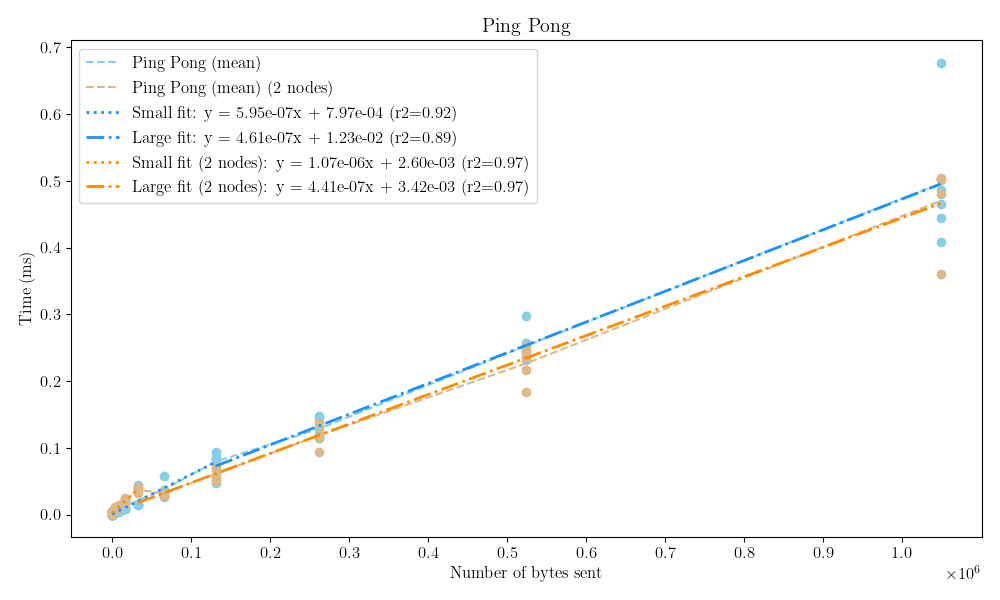
\includegraphics[width=\textwidth]{../fig/lab0/pingPong.png}
    \caption{Ping Pong: Number of bytes sent vs. average time taken from 1000 pairs of send / receive. 5 runs shown for each size as scatter plot. Mean of these 5 runs shown as line. Blue small fit includes all data points up to 131072 bytes, blue large from there. Red small fit includes all data points up to 32768 bytes, red large from there.}
    \label{fig:pingpong}
\end{figure}
As can be seen in the data and the fits, there are outliers especially for the larger data sizes. \\
For our runs we get the following fits and R² values:
\begin{table}[h!]
    \centering
    \begin{tabular}{|l|l|l|l|}
        \hline
        \textbf{Run Type}   & \textbf{Data Size} & \textbf{Fit Equation}                                      & \textbf{R² Value} \\ \hline
        \textbf{Single Node} & Small (<=131072)             & $5.95 \times 10^{-7} \cdot x + 7.97 \times 10^{-4}$        & 0.92              \\ \hline
        \textbf{Single Node} & Large (>= 131072)& $4.61 \times 10^{-7} \cdot x + 1.23 \times 10^{-2}$        & 0.89              \\ \hline
        \textbf{Two Node}    & Small (<=32768)& $1.07 \times 10^{-6} \cdot x + 2.60 \times 10^{-3}$        & 0.97              \\ \hline
        \textbf{Two Node}    & Large (>=32768)   & $4.41 \times 10^{-7} \cdot x + 3.42 \times 10^{-3}$        & 0.97              \\ \hline
    \end{tabular}
    \caption{Fit Equations and R² Values for Single Node and Two Node Runs}
\end{table}

\subsection{MM-product}

\setcounter{section}{-1}
\section{Appendix - Introduction }
\label{app:pingpong}
The following code was used for the ping pong task:
\lstinputlisting[language=c]{input/code/00/pingPong.c}
For the bonus task, the following code was used:
\lstinputlisting[language=c]{input/code/00/pingPongBonus.c}



